\documentclass[10pt,a4paper]{article}
\usepackage[margin=2cm]{geometry}
\usepackage{amsmath,amssymb}
\usepackage{graphicx,booktabs,xcolor}
\usepackage{listings}
\usepackage{tikz}
\usetikzlibrary{arrows.meta}
\usepackage[colorlinks=true,linkcolor=blue!50!black,urlcolor=blue!50!black,citecolor=blue!50!black]{hyperref}
\usepackage{microtype}

\lstset{language=Python,basicstyle=\ttfamily\small,keywordstyle=\color{blue!60!black}\bfseries,
  commentstyle=\color{green!40!black},stringstyle=\color{red!50!black},
  frame=single,framerule=0.3pt,rulecolor=\color{gray!60},backgroundcolor=\color{gray!5},
  columns=fullflexible,keepspaces=true,showstringspaces=false,
  numbers=left,numberstyle=\tiny\color{gray},xleftmargin=1.5em,aboveskip=6pt,belowskip=4pt}
\newcommand{\code}[1]{\texttt{#1}}
\newcommand{\cl}{\operatorname{cl}}
\newcommand{\st}{\operatorname{st}}
\newcommand{\lbr}{\char123 }\newcommand{\rbr}{\char125 }\newcommand{\tld}{\char126 }
%html \renewcommand{\lbr}{\{}\renewcommand{\rbr}{\}}\renewcommand{\tld}{\textasciitilde}
\newcommand{\prerel}{\text{an element of $r$ is a vertex, edge or face of an element of $s$}}
%html \renewcommand{\prerel}{\text{an element of }r\text{ is a vertex, edge or face of an element of }s}
\renewcommand{\labelitemi}{$\bullet$}
\newcommand{\incpic}{%
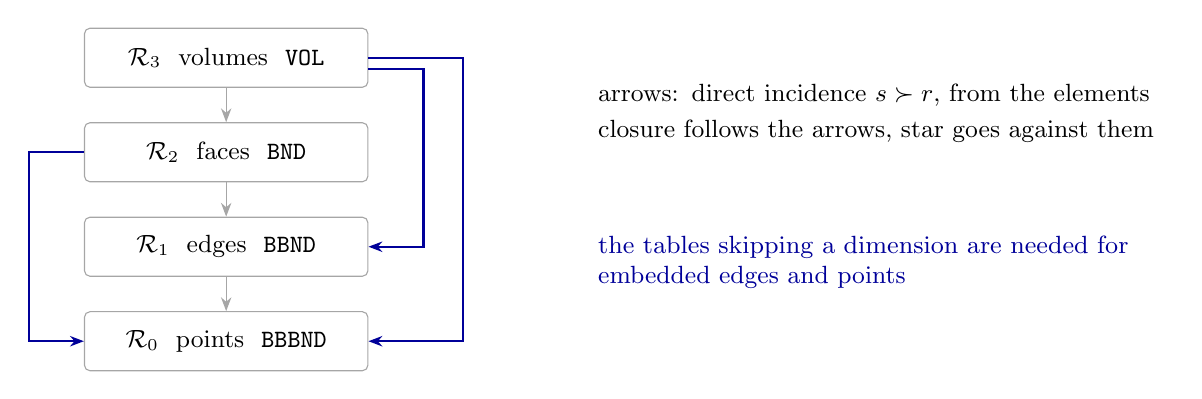
\begin{tikzpicture}[x=1cm,y=1cm,>={Stealth[length=5pt]},
  box/.style={draw=gray!70,rounded corners=2pt,minimum width=3.6cm,minimum height=0.75cm,font=\small}]
\node[box] (v) at (0,3.6) {$\mathcal R_3$\ \ volumes\ \ \code{VOL}};
\node[box] (f) at (0,2.4) {$\mathcal R_2$\ \ faces\ \ \code{BND}};
\node[box] (e) at (0,1.2) {$\mathcal R_1$\ \ edges\ \ \code{BBND}};
\node[box] (p) at (0,0.0) {$\mathcal R_0$\ \ points\ \ \code{BBBND}};
\draw[->,gray!70] (v) -- (f); \draw[->,gray!70] (f) -- (e); \draw[->,gray!70] (e) -- (p);
\draw[->,blue!60!black,thick] (v.east) -- ++(1.2,0) |- (p.east);
\draw[->,blue!60!black,thick] ([yshift=-4pt]v.east) -- ++(0.7,0) |- (e.east);
\draw[->,blue!60!black,thick] (f.west) -- ++(-0.7,0) |- (p.west);
\node[anchor=west,font=\small,text width=7.2cm] at (4.6,2.9)
  {arrows: direct incidence $s\succ r$, from the elements\\[2pt]
   closure follows the arrows, star goes against them};
\node[anchor=west,font=\small,text width=7.2cm,blue!60!black] at (4.6,1.0)
  {the tables skipping a dimension are needed for embedded edges and points};
\end{tikzpicture}}
%html \renewcommand{\incpic}{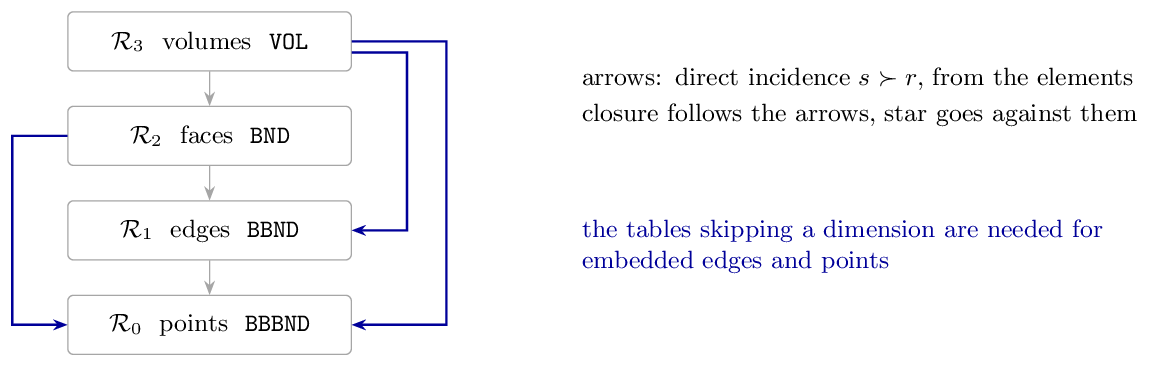
\includegraphics[width=0.8\textwidth]{incidence.png}}
\setlength{\parindent}{0pt}\setlength{\parskip}{4pt}\setlength{\emergencystretch}{3em}\sloppy
\setlength{\textfloatsep}{8pt}\setlength{\intextsep}{7pt}\setlength{\abovecaptionskip}{4pt}\setlength{\belowcaptionskip}{0pt}

\title{\vspace{-1.2cm}Mixed-dimensional Regions\\[2pt]
\large Selecting volumes, faces, edges and points of a mesh with one object}
\author{Christopher Lackner \and Joachim Sch\"oberl}
\date{NGSolve Technical Note 2026-06\quad$\bullet$\quad version 2026-11-17}

\begin{document}
\maketitle\vspace{-1.2cm}

\section{The problem}

The elements of a Netgen/NGSolve mesh \cite{s97,s14} carry a region index: volume elements a material, surface elements a boundary condition, segments an edge region, point elements a vertex region. A \code{Region} is a subset of the regions of \emph{one} of these four lists, identified by the codimension \code{VorB} $\in\{$\code{VOL}, \code{BND}, \code{BBND}, \code{BBBND}$\}$, and stored as a bit mask:
\begin{lstlisting}[numbers=none,xleftmargin=0pt]
mesh.Materials("iron|air")      mesh.Boundaries("outer")
mesh.BBoundaries("rail")        mesh.BBBoundaries("pin")
\end{lstlisting}
Many tasks need regions of several codimensions at once.
\begin{itemize}\setlength\itemsep{1pt}
\item \textbf{Essential boundary conditions.} A structure is clamped on a face, supported on an edge, and pinned in one point against a rigid body motion. So far this needed the three flags \code{dirichlet}, \code{dirichlet\_bbnd} and \code{dirichlet\_bbbnd}.
\item \textbf{Mixed-dimensional models.} A solid with a shell on a part of its surface and a beam along an edge; a multiplier on an interface; a coefficient with one value in a domain and another one on a boundary.
\item \textbf{Topology.} Which faces, edges and points belong to the boundary of a domain? What is the interface of two domains, including its rim? Where do two boundary conditions meet? The answers are sets of regions of different codimension.
\end{itemize}
The \code{MixedRegion} is one object for such a selection. With the region incidence of the mesh it also provides closure, boundary and star. This note describes the semantics, the data structures, and where a \code{MixedRegion} is accepted.

\section{The object}

A \code{MixedRegion} consists of a mesh and four bit masks, one for each \code{VorB}. It is created by the operator \code{|} between regions of different codimension, by regular expressions for the single codimensions, or from one \code{Region}. Wherever a \code{MixedRegion} is expected, a \code{Region} is converted automatically.
\begin{lstlisting}[numbers=none,xleftmargin=0pt]
clamp = mesh.Boundaries("bot") | mesh.BBoundaries("rail") | mesh.BBBoundaries("pin")
clamp = mesh.MixedRegion(BND="bot", BBND="rail", BBBND="pin")              # the same
print (clamp)                 # MixedRegion(BND: [bot], BBND: [rail], BBBND: [pin])
\end{lstlisting}
The operations are those of sets, applied to each mask (Table~\ref{tab:ops}). Operands must belong to the same mesh object.

\begin{table}[h]\centering\small
\begin{tabular}{@{}lll@{}}\toprule
operation & result & remark\\\midrule
\code{a | b},\ \code{a \& b},\ \code{a - b},\ \code{\tld a} & \code{MixedRegion} & set operations in each codimension\\
\code{a[VOL]}, \code{a[BND]}, \dots & \code{Region} & the part of one codimension\\
\code{a.Closure()} & \code{MixedRegion} & \code{a} and all lower-dimensional regions it touches\\
\code{a.Boundary()} & \code{MixedRegion} & the regions one dimension lower which \code{a} touches\\
\code{a.Star()} & \code{MixedRegion} & \code{a} and all higher-dimensional regions touching it\\
\code{a.IsClosed()}, \code{a.Empty()}, \code{a == b} & \code{bool} & \\
\code{a.IndicatorCF()} & \code{CoefficientFunction} & $1$ on the elements of \code{a}, else $0$\\
\bottomrule\end{tabular}
\caption{Operations of a \code{MixedRegion}.}\label{tab:ops}
\end{table}

\textbf{Open sets.} A \code{MixedRegion} contains exactly the regions which were given. A face does not bring its edges along. The closure is an operation of its own, and every function which takes a \code{MixedRegion} documents whether it adds lower-dimensional parts. The reason is that there is no single right answer: the dofs of a continuous space on a face include those on its edges, the dofs of a discontinuous or a facet space do not.

\textbf{Two types.} The operators of \code{Region} are unchanged: \code{+}, \code{-}, \code{*} combine regions of the same codimension and return a \code{Region}; for regions of different codimension or of different meshes they now throw an exception (before, the masks of two unrelated lists were combined silently). The operator \code{|} returns a \code{Region} for two regions of the same codimension, and a \code{MixedRegion} otherwise. A \code{Region} and a \code{MixedRegion} never compare equal.

\textbf{Descriptors without a mesh.} \code{VOL("ball")}, \code{BND("bot")}, \code{BBND("rail")}, \code{BBBND("pin")} name regions of one codimension, and \code{|} combines them into a \code{MixedRegionDescriptor}: names per codimension, regular expressions as before, no mesh. The mesh resolves it, \code{descr[BND]} gives the part, and descriptors pickle.
\begin{lstlisting}[numbers=none,xleftmargin=0pt]
descr = BND("bot") | BBND("rail") | BBBND("pin")      # BND(bot) | BBND(rail) | BBBND(pin)
mr = mesh[descr]            # MixedRegion; equals the union of the three
descr[BND], descr[VOL]      # BND(bot), None
\end{lstlisting}
A descriptor is accepted by the functions of Table~\ref{tab:use} (\code{dirichlet}, \code{definedon}, keys of \code{RegionCF}, \code{u[...] == g}, \code{gf[...] = cf}). Two descriptors of the same codimension give a plain region descriptor.

\section{Region incidence}\label{sec:inc}

Let $\mathcal R_d$ be the set of regions of entity dimension $d\in\{0,1,2,3\}$, i.e.\ vertex, edge, face and volume regions. In a mesh of dimension $D$ the codimension $v$ corresponds to $d = D-v$. For $r\in\mathcal R_d$ and $s\in\mathcal R_{d'}$ with $d<d'$ we write
\[
r \prec s \quad :\Longleftrightarrow\quad \prerel.
\]
For a set $M$ of regions
\[
\cl M = M\cup\{r: r\prec s,\ s\in M\},\qquad
\st M = M\cup\{s: r\prec s,\ r\in M\},\qquad
\partial M = \{r\in\mathcal R_{d-1}: r\prec s,\ s\in M\cap\mathcal R_d\}.
\]

\textbf{Direct tables.} The relation is stored for all six pairs $d<d'$, in both directions, and not composed from the pairs of neighbouring dimensions. An edge region inside of a volume (a wire, a beam, a line source) or a point region inside of a face touches the higher-dimensional region without lying on a region of the dimension in between; a composition $\mathcal R_3\to\mathcal R_2\to\mathcal R_1$ would miss it (Figure~\ref{fig:inc}).

\begin{figure}[h]\centering
\incpic
\caption{Region incidence for a mesh of dimension $3$. All six tables are built from elements.}\label{fig:inc}
\end{figure}

\textbf{Computation.} The tables are computed in Netgen, \code{Mesh::GetRegionIncidence()}, indexed by the entity dimension like the region descriptors \code{Region<D>} of the mesh. With the topology of the mesh, three maps are built: vertex $\to$ regions of its point elements, edge $\to$ regions of its segments, face $\to$ regions of its surface elements. An entity may belong to several regions. One loop over the segments, the surface elements and the volume elements then looks up their vertices, edges and faces in these maps. The cost is one pass over the elements. Netgen computes the tables at each call, from the current elements; nothing is cached there. NGSolve fetches them once after each update of the mesh (\code{MeshAccess::BuildNeighbours}); the existing functions \code{Region.Neighbours(vb)} and \code{Region.Boundaries()} use the same tables. In Python the tables are available as \code{mesh.ngmesh.RegionIncidence(d1,d2)}.

\textbf{What the closure sees.} The relation is defined by elements. An edge of the geometry without segments in the mesh is not a region and not seen by the closure. Meshes from OCC geometries have segments for all edges and point elements for all vertices of the geometry.

\textbf{Limits.} The incidence is not stored in the mesh and not written to the \code{.vol} file; it is computed from the elements at each call and needs valid edge and face tables. Regions exist only where the mesh has elements of that dimension. Two regions are incident if one pair of elements touches, which equals the B-rep topology for OCC meshes. It is known per MPI rank only. Hand-made meshes work.

\textbf{One step.} $\cl$ adds the regions directly below $M$. If every region is one entity of a boundary representation (one face, one edge, one vertex, as for OCC geometries), then $r\prec s\prec t$ implies $r\prec t$, and $\cl\cl M = \cl M$. For regions which are unions of unrelated pieces (one boundary condition number for several patches of an imported mesh) this need not hold: $r$ may touch $s$ in one place and $s$ touch $t$ in another one. \code{IsClosed()} tests $\cl M = M$.

\section{Where a MixedRegion is accepted}

\begin{table}[h]\centering\small
\begin{tabular}{@{}lll@{}}\toprule
function & meaning for a \code{MixedRegion} & adds lower dimensions?\\\midrule
\code{FESpace(..., dirichlet=mr)} & constrain the dofs of the \code{BND}, \code{BBND}, \code{BBBND} parts & as the space does for elements\\
\code{FESpace(..., definedon=mr)} & like the dict \code{\lbr VOL: ..., BND: ...\rbr} & yes, all sub-entities (Sec.~\ref{sec:def})\\
\code{fes.GetDofs(mr)}, \code{u.GetDofs(mr)} & union of the dofs of the elements of all parts & no\\
\code{mesh.RegionCF(\lbr mr: value\rbr)} & value in all non-empty parts of \code{mr} & no\\
\code{mr.IndicatorCF()} & see Table~\ref{tab:ops} & no\\
\code{u[mr] == g} in \code{Solve} & Dirichlet condition on all parts & as \code{dirichlet}\\
\code{gf[mr] = cf} & set the dofs of the parts to \code{cf} & see example\\
\bottomrule\end{tabular}
\caption{Functions taking a \code{MixedRegion} or a descriptor.}\label{tab:use}
\end{table}

\textbf{Dirichlet.} The parts are combined by \emph{or} with the flags \code{dirichlet\_bbnd} and \code{dirichlet\_bbbnd}, which keep working. A volume part is an error. A plain \code{Region} of \code{BBND} or \code{BBBND} is accepted as well (\code{dirichlet=mesh.BBoundaries("rail")}); a non-empty \code{VOL} region is an error. \code{dirichlet=BBND("rail")} and \code{dirichlet\_bbnd="rail"} give the same free dofs. A dof is constrained if it belongs to an element of a selected region; for $H^1$ and $H(\operatorname{curl})$ spaces a face therefore constrains the dofs on its edges and vertices as before, without a closure. What is new is that an isolated edge or point is given in the same argument.

\textbf{Compact syntax.} \code{Solve(a == f, u[BND("left") | BBND("edge")] == g, pre, solver)} takes a descriptor (also \code{BND("bot")} alone); the condition keeps it (\code{bc.vbn}). It was run with \code{BDDC} and \code{CGSolver}; the solution equals that of the flag form to $10^{-16}$.

\textbf{Coefficients.} \code{mesh.RegionCF(\lbr region: value, ...\rbr, default=...)} without a \code{VorB} takes regions of any codimension as keys. It is one \code{CoefficientFunction}; the codimension of the element selects the list of values, the region index the entry. A \code{MixedRegion} as key sets the value in each of its non-empty parts. The \code{default} applies to the remaining regions of those codimensions which have a given region; in the other codimensions the function is undefined, and the use there is refused before any element is touched. The region-wise functions \code{MaterialCF}, \code{BoundaryCF} and \code{RegionCF} are now one class (\code{RegionCoefficientFunction}, C.~Lackner); pickles of the former class \code{DomainWiseCoefficientFunction} written since version 6.2.2406 can be loaded.

\textbf{Not an integration domain.} \code{dx(definedon=...)}, \code{ds(definedon=...)} and \code{Integrate(..., definedon=...)} take a \code{Region}. The measure and usually the integrand depend on the codimension, so an integral over a \code{MixedRegion} is not defined. Use the parts: \code{dx(definedon=mr[VOL])}.

\section{Defined-on and Dirichlet regions of a space}\label{sec:def}

\textbf{The flag is closed.} For every form of \code{definedon} (\code{Region}, \code{MixedRegion}, descriptor, string, dict \code{\lbr VOL: ..., BND: ...\rbr}) the space is defined on the given regions and all their sub-entities: each lower-dimensional mask is what was given, united with the closure of everything given above it. Before, edges and points were either unrestricted or exactly the given part. The dof numbering does not change. What changes is where edge and point terms are assembled and where a \code{GridFunction} counts as defined. With MPI the closed masks are OR-reduced over the ranks, since the incidence is known per rank only.
\begin{lstlisting}[numbers=none,xleftmargin=0pt]
fs = H1(mesh, order=2, definedon=mesh.Boundaries("top"))
MixedRegion(mesh.Boundaries("top")).Closure() == fs.definedon     # True
\end{lstlisting}

\textbf{Storage.} The space keeps both sets as \code{MixedRegion}. In Python \code{fes.definedon} and \code{fes.dirichlet} are read-only copies; \code{fes.GetDefinedOnRegion(vb)} equals \code{fes.definedon[vb]}, and for an unrestricted space \code{fes.definedon == \tld MixedRegion(mesh)}. In C++:
\begin{itemize}\setlength\itemsep{1pt}
\item members \code{definedon\_region}, \code{dirichlet\_region}; all four masks always have full size, ``everywhere'' means all bits set (before: empty array);
\item \code{DefinedOnAll(vb)}; \code{GetDefinedOn(vb)} and \code{DefinedOn(vb)} return \code{BitArray} (before: \code{Array<bool>}); \code{DefinedOnX} is removed;
\item the archive layout is unchanged; \code{Update} resizes the masks of an unrestricted space if the number of regions changed, and throws for a restricted one.
\end{itemize}

\textbf{Elements without region.} A segment added by hand without edge index (\code{Element1D(..., index=0)} in a 3D mesh) is a \code{BBND} element with region index $-1$. It belongs to no region: the space is not defined on it (\code{GetDofNrs} is empty) and it gets no Dirichlet dofs.

\section{Example}

A unit cube contains a ball. The solution is fixed on the bottom face, on one edge of the top face, and in one corner. The coefficient is $1$ in the cube, $10$ in the ball, and the same function gives the Robin coefficient $5$ on the top face.

\begin{lstlisting}
from ngsolve import *
from netgen.occ import *

box = Box((0,0,0), (1,1,1))
box.solids.name = "air";  box.faces.name = "wall"
box.faces.Min(Z).name = "bot";  box.faces.Max(Z).name = "top"
box.edges.Max(X+Z).name = "rail"
box.vertices.Max(X+Y+Z).name = "pin"
ball = Sphere((0.5,0.5,0.5), 0.25)
ball.solids.name = "ball";  ball.faces.name = "sphere"
mesh = Mesh(OCCGeometry(Glue([box-ball, ball])).GenerateMesh(maxh=0.2))

clamp = mesh.Boundaries("bot") | mesh.BBoundaries("rail") | mesh.BBBoundaries("pin")
fes = H1(mesh, order=2, dirichlet=clamp)              # ndof = 2089, 1937 free dofs
# same as  H1(mesh, order=2, dirichlet="bot", dirichlet_bbnd="rail", dirichlet_bbbnd="pin")

k = mesh.RegionCF({mesh.Materials("air"): 1, mesh.Materials("ball"): 10,
                   mesh.Boundaries("top"): 5}, default=0)
u, v = fes.TnT()
a = BilinearForm(k*grad(u)*grad(v)*dx + k*u*v*ds).Assemble()
f = LinearForm(v*dx).Assemble()
gfu = GridFunction(fes)
gfu.vec.data = a.mat.Inverse(fes.FreeDofs()) * f.vec  # mean value 0.1184

# topology
cball = MixedRegion(mesh.Materials("ball")).Closure()
cball[BND] == mesh.Boundaries("sphere")                         # True
iface = MixedRegion(mesh.Materials("air")).Closure() & cball    # the sphere, no volume
MixedRegion(mesh.BBBoundaries("pin")).Star()   # 1 volume, 3 faces, 3 edges, the point
ind = clamp.IndicatorCF()
Integrate(ind, mesh, BND), Integrate(ind, mesh, BBND)           # 1.0, 1.0: area, length
\end{lstlisting}
The matrix \code{a} equals the one assembled with a \code{MaterialCF} in the volume term and the boundary term \code{5*u*v*ds("top")}; the two solutions agree to the last digit. The coefficient \code{k} is $0$ on the boundaries other than \code{top} by the \code{default}.

Descriptors, the closed flag and elements without region:
\begin{lstlisting}
descr = BND("bot") | BBND("rail") | BBBND("pin")
fes = H1(mesh, order=2, dirichlet=descr)          # 2089 dofs, 1937 free: as clamp above
gf = GridFunction(fes);  gf[descr] = 3      # 3.0 at (.3,.3,0) and (1,1,1), 0 at (.1,.1,.9)
k = mesh.RegionCF({VOL("air"): 1, VOL("ball"): 10,
                   BND("top") | BBND("rail"): 5}, default=0)
Integrate(k, mesh, BND), Integrate(k, mesh, BBND)     # 5.0, 5.0
u, v = fes.TnT()
gs = Solve(grad(u)*grad(v)*dx + u*v*ds("top") == 1*v*dx, u[descr] == 0)
H1(mesh, order=2, dirichlet=mesh.BBoundaries("rail"))   # 2078 free of 2089
H1(mesh, order=2, dirichlet=mesh.Materials("ball"))     # NgException: VOL regions are not supported
\end{lstlisting}
In a tetrahedron with two hand-made segments, one with index $0$ (region $-1$) and one with index $1$, \code{H1(order=1)} has dof counts \code{[0, 2]} on the two segments, and \code{dirichlet\_bbnd=".*"} leaves \code{[True, True, False, False]} free.

\section{Rules and pitfalls}

\begin{itemize}\setlength\itemsep{1pt}
\item \textbf{The mesh object matters.} Regions belong to one \code{Mesh} object. Regions of two \code{Mesh} objects are not combined, also if both wrap the same Netgen mesh or one is the unpickled copy of the other. Pickle a region together with its mesh.
\item \textbf{After a change of the mesh.} The masks have the sizes of the region lists at the time of creation. Refinement keeps the regions; after a change of the region lists a stored region is rejected by the flags of the spaces and by \code{RegionCF}.
\item \textbf{Empty parts.} An empty part of a \code{MixedRegion} does not stand for its codimension: as a key of \code{RegionCF} it does not activate the \code{default} there, and a completely empty key is an error. A mistyped name gives an empty \code{Region} without a message, as before.
\item \textbf{One region around two materials.} Incidence is by regions. A boundary region running around two materials makes a space with \code{definedon} one material defined on the whole boundary region. In a 2D mesh of $4\times4$ quadrilaterals with materials \code{left}, \code{right} and one boundary region \code{outer}, \code{H1(order=2, definedon=mesh.Materials("left"))} has 63 dofs, 60 of them used, and 15 used dofs have a zero diagonal in \code{u*v*dx} (no volume element on the far part). With \code{outer\_l} and \code{outer\_r} instead: 55 dofs, 45 used, no zero row. Remedy: one boundary region per material.
\item \textbf{Boundary is incidence.} \code{Boundary()} contains the interface between two selected domains. There is no orientation, and no relation like $\partial\partial = 0$.
\item \textbf{Parallel meshes.} The incidence is computed from the elements of each rank. Closure, boundary and star may differ between the ranks, as \code{Region.Neighbours} did before. The masks and \code{dirichlet} are not affected; the closed \code{definedon} masks are OR-reduced over the ranks.
\end{itemize}

\section{Related work and outlook}

Regions of all dimensions with a closure are the labels of PETSc DMPlex \cite{ks09,lmkg16}, where a label marks mesh points of any dimension and boundary conditions act on the closure of a label. The difference is the level: DMPlex stores the cell complex of the mesh entities, the region incidence of Section~\ref{sec:inc} is the complex of the geometric entities, which is small and independent of refinement. A closed \code{MixedRegion} is a subcomplex in the sense of finite element exterior calculus \cite{afw06}; essential conditions on it lead to the relative de Rham complex.

Further functions are planned to take a \code{MixedRegion}: marks for singular points, edges and faces in $hp$-refinement, extraction of a submesh with its lower-dimensional regions, selection of additional coarse dofs in BDDC, and local mesh size.

\textbf{Status.} The features are in the NGSolve master branch since November 2026.

{\small
\begin{thebibliography}{9}\setlength{\itemsep}{1pt}
\bibitem{s97} J.~Sch\"oberl. NETGEN: An advancing front 2D/3D-mesh generator based on abstract rules. \emph{Comput. Vis. Sci.} 1(1):41--52, 1997.
\bibitem{s14} J.~Sch\"oberl. C++11 implementation of finite elements in NGSolve. ASC Report 30/2014, TU Wien, 2014.
\bibitem{ks09} M.~G.~Knepley and D.~A.~Karpeev. Mesh algorithms for PDE with Sieve I: Mesh distribution. \emph{Sci. Program.} 17(3):215--230, 2009.
\bibitem{lmkg16} M.~Lange, L.~Mitchell, M.~G.~Knepley and G.~J.~Gorman. Efficient mesh management in Firedrake using PETSc DMPlex. \emph{SIAM J. Sci. Comput.} 38(5):S143--S155, 2016.
\bibitem{afw06} D.~N.~Arnold, R.~S.~Falk and R.~Winther. Finite element exterior calculus, homological techniques, and applications. \emph{Acta Numer.} 15:1--155, 2006.
\end{thebibliography}}

\end{document}
